\documentclass{article}
\usepackage[utf8]{inputenc} % Permite el uso de caracteres del Español
\usepackage[T1]{fontenc}
\usepackage{hyperref}
\usepackage{graphicx}
\usepackage{wrapfig}
\usepackage{subcaption}

% set font encoding for PDFLaTeX or XeLaTeX
\usepackage{ifxetex}
\ifxetex
  \usepackage{fontspec}
\else
  \usepackage[T1]{fontenc}
  \usepackage[utf8]{inputenc}
  \usepackage{lmodern}
\fi

% used in maketitle
\title{Actividad 4: Introducción a la programación de los intérpretes de comandos}
\author{Melissa Matrecitos Avila}
\date{26 de Febrero de 2018}

% Enable SageTeX to run SageMath code right inside this LaTeX file.
% documentation: http://mirrors.ctan.org/macros/latex/contrib/sagetex/sagetexpackage.pdf
% \usepackage{sagetex}

\begin{document}
\maketitle

\section{Introducción}
El siguiente texto es el reporte de la actividad 4 del curso de Física Computacional 1, en la cual se trabajó con un interprete de comandos llamado Shell, el es una interfaz de usuario para acceder a los servicios de un sistema operativo, en este caso LINUX.

En esta actividad trabajamos las distintas formas de interactuar y hacer scripts (programas) con el Shell (/bin/sh) y el  Again Shell (/bin/bash). Para llevarla a cabo se utilizaron los comandos cat, chmod, echo, grep, less, ls y wc, los cuales se explicaran en los resultados de la práctica.

Por último se realizó una síntesis sobre las notas de Steve Parker "Shell Script Tutorial", de los cuales se incluyen ejemplos de las secciones que allí vienen.

\section{Síntesis}
En esta sección se presentará la sítesis sobre las notas de Steve Parker "Shell Script Tutorial" con algunos ejemplos.
\subsection{Introducción y Filosofía}
Este tutorial está escrito para ayudar a las personas a comprender algunos de los conceptos básicos de la programación de scripts de shell.
Hay una serie de factores que pueden incluirse en scripts de shell buenos, limpios y rápidos.
\begin{itemize}
\item Los criterios más importantes deben ser un diseño claro y legible.
\item La segunda es evitar comandos innecesarios.
\end{itemize}
Un diseño claro hace la diferencia entre un guión de shell que aparece como "magia negra" y uno que se mantiene y comprende fácilmente.
\subsection{Un Primer Script}
Para el primer script se escribirá uno que diga "Hello World", esto se logra, primero que nada especificando por quien debe ser ejecutado el script y con el comando echo se escribe en la pantalla los argumentos que lo acompañan. Es importante saber que echo pondrá automáticamente un espacio entre los argumentos, para evitarlo, el argumento se debe escribir entre comillas, otra cosa importante es saber que el símbolo  \# es para agregar comentarios, excepto cuando es acompañado de ! ya que \#! significa que lo que sigue debe ser interpretado por el shell de Bourne.

\begin{verbatim}
#!/bin/bash
#Comentario
echo Hello World
\end{verbatim}

\begin{verbatim}
#!/bin/bash
#Comentario
echo"Hola    Mundo"
\end{verbatim}

\subsection{Variables Parte 1}
Casi todos los lenguajes de programación existentes tienen el concepto de variables , un nombre simbólico para un trozo de memoria al que podemos asignar valores, leer y manipular sus contenidos.
Tenga en cuenta que no debe haber espacios alrededor del signo "=", el cual tarta el comando como una asignación de variable.

Al shell no le importan los tipos de variables; pueden almacenar cadenas, enteros, números reales, cualquier cosa que te guste. Podemos establecer de manera interactiva nombres de variables usando el readcomando.

No es necesario declarar las variables en el shell Bourne, como sí lo hacen en lenguajes como C. Pero si intenta leer una variable no declarada, el resultado es la cadena vacía. No obtienes advertencias o errores.

\begin{verbatim}
#!/bin/bash
echo "Hola, ¿Cómo te llamas?"
read Nombre
echo "¿Cuál es tu color favorito, $Nombre?"
read Color
echo "El color favorito de $Nombre es $Color"
\end{verbatim}

\begin{verbatim}
#!/bin/bash
echo "Hola, para saber el año en el que naciste escribe el año actual:"
read Actual
echo "¿Cuál será tu edad este año?"
read Edad
echo "El año en que naciste es"
expr $Actual-$Edad
\end{verbatim}

\subsection{Comodines}
Los comodines no son muy útiles en los scripts de shell. Esta sección es realmente solo para mover y editar archivos en la terminal. Son más utilizados cuando hay ciclos.
\begin{verbatim}
#!/bin/bash
#Copiar archivos de a hacía b
cp / tmp / a / * / tmp / b /
\end{verbatim}

\begin{verbatim}
#!/bin/bash
#Escribir lo que contiene la carpeta a
echo /tmp/a/*
\end{verbatim}

\subsection{Caracteres de Escape}
La mayoría de los caracteres ( *, ', etc) no se interpretan (es decir, que se toman literalmente)  a menos de que sean colocados entre comillas dobles (""). Pero para los caracteres ", $, `, y \ siguen siendo interpretado cómo código a pesar de las comillas, para esto se utiliza caracter de barra invertida (\) el cual hace que el intérprete no los interprete, sino que los pase al comando que se esta utilizando.

\begin{verbatim}
#!/bin/bash
echo "Tienes que pagar \$ 10. "
\end{verbatim}

\begin{verbatim}
#!/bin/bash
echo "Mi nombre es \"Melissa\" "
\end{verbatim}

\subsection{Ciclos}
La mayoría de los lenguajes tienen el concepto de bucles: si queremos repetir una tarea veinte veces, no queremos tener que escribir el código veinte veces, con un ligero cambio cada vez.
Como resultado, tenemos fory whilebucles en el shell Bourne.

Los bucles "for" iteran a través de un conjunto de valores hasta que se agote la lista:
\begin{verbatim}
#!/bin/bash
for i in 10, 9, 8, 7, 6, 5, 4, 3, 2, 1
do
  echo "Summer"
done
  echo"What time is it ? Summertime!"
\end{verbatim}

Los bucles "while" iteran hasta que se cumpla una condición de salida, éste tipo de bucles se dice que son más "divertidos" debido a que el usuario decide si va a seguir dentro o va a salir del ciclo:
\begin{verbatim}
#!/bin/bash
salida=Halo
while [ "$salida" != "Tschüss" ]
do
  echo "Escribe algo (Tschüss para salir)"
  read salida
  echo "Escribiste: $salida"
done
\end{verbatim}

\subsection{Prueba (test)}
\textbf{"["} es un enlace simbólico de test, solo para hacer que los programas shell sean más legibles. Esto significa que "test" es en realidad un programa, al igual que ls u otros programas. 
Test a menudo se invoca indirectamente a través de las instrucciones if y while. También es la razón por la que tendrás problemas si creas un programa llamado testy tratas de ejecutarlo, ya que se llamará a este intérprete de comandos en lugar de tu programa.
\begin{verbatim}
#!/bin/bash
echo -en "Please guess the magic number: "
read X
echo $X | grep "[^0-9]" > /dev/null 2>&1
if [ "$?" -eq "0" ]; then
  # If the grep found something other than 0-9
  # then it's not an integer.
  echo "Sorry, wanted a number"
else
  # The grep found only 0-9, so it's an integer.
  # We can safely do a test on it.
  if [ "$X" -eq "7" ]; then
    echo "You entered the magic number!"
  fi
fi
\end{verbatim}

\begin{verbatim}
#!/bin/bash
X=0
while [ -n "$X" ]
do
  echo "Enter some text (RETURN to quit)"
  read X
  if [ -n "$X" ]; then
    echo "You said: $X"
  fi
done
\end{verbatim}

\subsection{Caso}
La "case" declaración guarda pasar por un conjunto completo de if .. then .. else declaraciones. Pueden ser una herramienta muy útil y poderosa. A menudo se utilizan para analizar los parámetros pasados a un script de shell, entre otros usos.
\begin{verbatim}
#!/bin/bash
echo "Please talk to me ..."
while :
do
  read INPUT_STRING
  case $INPUT_STRING in
	hello)
		echo "Hello yourself!"
		;;
	bye)
		echo "See you again!"
		break
		;;
	*)
		echo "Sorry, I don't understand"
		;;
  esac
done
echo
echo "That's all folks!"
\end{verbatim}

\subsection{Variables Parte 2}
Ya hay un conjunto de variables establecidas para usted, y la mayoría de ellas no pueden tener valores asignados. 
Estos pueden contener información útil, que el script puede utilizar para conocer el entorno en el que se está ejecutando. 
El primer conjunto de variables que veremos son \$0 .. \$9 y \$\#. 
La variable \$0 es el nombre base del programa como se lo llamó. 
\$1 .. \$9 son los primeros 9 parámetros adicionales con los que se invocó el script. 

La variable \$@ es todos los parámetros \$1 .. cualquiera. La variable \$*, es similar, pero no conserva ningún espacio en blanco, y las comillas, por lo que "Archivo con espacios" se convierte en "Archivo" "con" "espacios". Como regla general, usa \$@y evita \$*. 

\$\# es la cantidad de parámetros con los que se invocó el script.
Otra variable es interesante IFS. Este es el separador de campo interno . El valor predeterminado es SPACE TAB NEWLINE, pero si lo está cambiando, es más fácil tomar una copia
Otra variable especial es \$?. Esto contiene el valor de salida del último comando de ejecución, esto ayuda a que los scripts sean robustos y más inteligentes.
\begin{verbatim}
#!/bin/bash
old_IFS="$IFS"
IFS=:
echo "Please input some data separated by colons ..."
read x y z
IFS=$old_IFS
echo "x is $x y is $y z is $z"
\end{verbatim}

\begin{verbatim}
#!/bin/bash
/usr/local/bin/my-command
if [ "$?" -ne "0" ]; then
  echo "Sorry, we had a problem there!"
fi
\end{verbatim}

\subsection{Variables Parte 3}
Como mencionamos en Variables - Parte I , las llaves alrededor de una variable evitan confusiones. Sin embargo, eso no es todo, estos brackets de lujo tienen otro uso mucho más poderoso. Podemos tratar con problemas de variables indefinidas o nulas.
\begin{verbatim}
#!/bin/bash
foo=sun
echo $fooshine     # $fooshine is undefined
echo ${foo}shine   # displays the word "sunshine"
\end{verbatim}

\begin{verbatim}
#!/bin/bash
echo -en "What is your name [ `whoami` ] "
read myname
if [ -z "$myname" ]; then
  myname=`whoami`
fi
echo "Your name is : $myname"
\end{verbatim}

\subsection{Programas externos}
Los programas externos a menudo se usan en scripts de shell; hay algunas órdenes internas ( echo, which, y test son comúnmente incorporados), pero muchos comandos útiles son en realidad utilidades Unix, tales como tr, grep, expry cut. El backtick (`) también se asocia a menudo con comandos externos, se usa para indicar que el texto adjunto se debe ejecutar como un comando.
\begin{verbatim}
#!/bin/bash
grep "^${USER}:" /etc/passwd | cut -d: -f5
\end{verbatim}

\begin{verbatim}
#!/bin/bash
MYNAME=`grep "^${USER}:" /etc/passwd | cut -d: -f5`
echo $MYNAME
\end{verbatim}

\subsection{Funciones}
Una característica que a menudo se pasa por alto de la programación de guiones de shell de Bourne es que puede escribir fácilmente funciones para usar en su secuencia de comandos. Esto generalmente se hace de una de dos maneras; con un script simple, la función simplemente se declara en el mismo archivo como se llama. 
Sin embargo, al escribir un conjunto de secuencias de comandos, a menudo es más fácil escribir una "biblioteca" de funciones útiles, y el origen de ese archivo al inicio de los otros scripts que utilizan las funciones.
Una función puede devolver un valor en una de cuatro formas diferentes:
\begin{itemize}
\item Cambiar el estado de una variable o variables
\item Use el exit comando para finalizar el script de shell
\item Utilice el return comando para finalizar la función y devolver el valor proporcionado a la sección de llamada del script de shell
\item echo output to stdout, que será capturado por la persona que lo llama al igual que c=`expr \$ a + \$ b` es llamado.
\end{itemize}
La diferencia es que una función de shell no puede cambiar sus parámetros, aunque puede cambiar los parámetros globales.
\begin{verbatim}
#!/bin/bash

myfunc()
{
  echo "I was called as : $@"
  x=2
}

### Main script starts here

echo "Script was called with $@"
x=1
echo "x is $x"
myfunc 1 2 3
echo "x is $x"
\end{verbatim}
\begin{verbatim}
#!/bin/bash

factorial()
{
  if [ "$1" -gt "1" ]; then
    i=`expr $1 - 1`
    j=`factorial $i`
    k=`expr $1 \* $j`
    echo $k
  else
    echo 1
  fi
}


while :
do
  echo "Enter a number:"
  read x
  factorial $x
done
\end{verbatim}

\subsection{Consejos y Sugerencias}
En esta sección, cómo lo dice su título, se nos brindan algunas sugerencias o tips sobre como mejorar los scrpits, como los dos ejemplos que se muestran a continuación:

\begin{verbatim}
#!/bin/bash
steves = `grep -i steve / etc / passwd | cut -d: -f1` 
echo "Todos los usuarios con la palabra" steve "en su passwd" 
echo "Las entradas son:" 
echo "$ steves" | tr '' '\ 012'
\end{verbatim}

\begin{verbatim}
#!/bin/bash
NO_LINES = `wc -l archivo | awk '{print $ 1}' `
\end{verbatim}

Se les dio mayor importancia a los que eran de tipo:
\begin{itemize}
\item CGI Scripting

\item Códigos de salida y control de flujo

\item Simple esperar reemplazo

\item Usar la trampa para saber cuándo te han interrumpido, como CTRL-C, etc.

\item Solución para la dicotomía 'echo -n' versus 'echo \ c'
\end{itemize}

\subsection{Referencia Rápida}
Se muestra una guía de referencia rápida sobre el significado de algunos de los comandos y códigos menos fáciles de adivinar de los scripts de shell. Por su naturaleza, también son bastante difíciles de encontrar usando los motores de búsqueda.
\begin{center}
 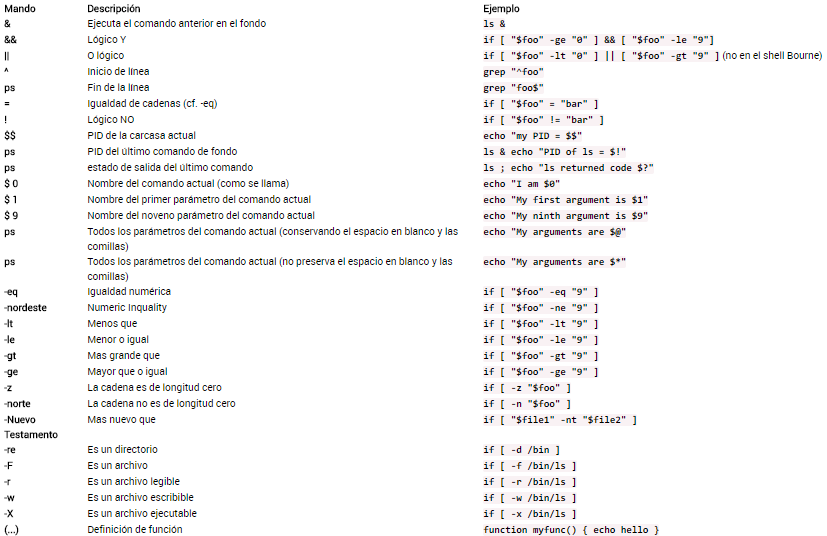
\includegraphics[width=1\textwidth]{referencias.PNG}
\end{center}


\subsection{Shell Interactivo}
Aquí hay algunas sugerencias rápidas para usar el shell UNIX o Linux de forma interactiva.

\begin{itemize}
\item bash:
tiene algunas herramientas de búsqueda de historia muy prácticas; las teclas de flecha hacia arriba y hacia abajo se desplazarán por el historial de comandos anteriores. Más útilmente, Ctrl + r hará una búsqueda inversa, haciendo coincidir cualquier parte de la línea de comando. Presione ESC y el comando seleccionado se pegará en el shell actual para que pueda editarlo según sea necesario.
\item ksh:
Puede hacer que ksh sea más útil agregando comandos de historial, ya sea en vi o emacs. Hay varias maneras de hacerlo, dependiendo de las circunstancias exactas: "set -o vi", o "ksh -o vi", o "exec ksh -o vi" (donde "vi" podría reemplazarse por "emacs" si prefiere el modo emacs). Además si golpeas ESC y k, al golpear repetidamente k, retrocedes en el historial de comandos. Puede usar los comandos vi command-mode y entry-mode para editar los comandos.
\end{itemize} 


\section{Resultados de la práctica}
A continuación se describirá la practica realizada:
Después de crear la carpeta "Actividad 4"en la cual se guardarían todos los archivos utilizados, se decargó el archivo proporcionado por el profesor llamado "script1.sh", en el cual se hicieron los cambios pertinentes para descargar los datos de la estación 10393, correspondiente a Linderburg en Alemania. Después con el comando \textbf{''chmod''} se creó el ejecutable de dicho script que se confirmo utilizando el comando \textbf{''ls -alg''}, que después se ejecutó en la terminal. Los 12 archivos descargados fueron:
\begin{center}
 
\includegraphics[width=0.8\textwidth]{archivosdescargados.png}

 Archivos descargados por el script1.sh
\end{center}

\begin{center}
  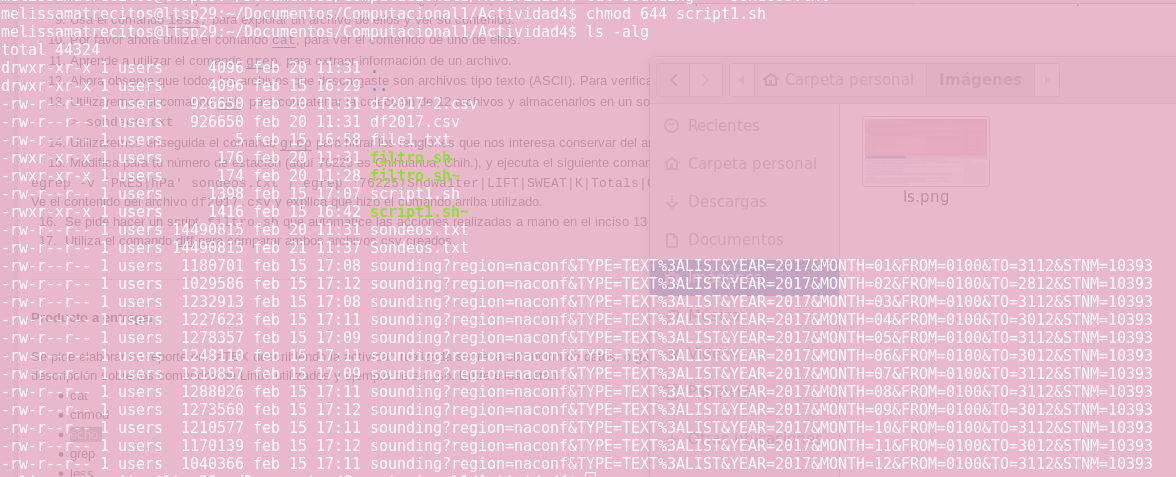
\includegraphics[width=0.8\textwidth]{chmod.png}

Comandos "chmod" y "ls-alg" en la terminal

\end{center}

Posteriormente con el comando \textbf{"less"} se exploró el archivo correspondiente al mes de febrero, este mostró el archivo en la terminal, ubicando el puntero al inicio del archivo:

\begin{center}

 
\includegraphics[width=0.99\textwidth]{less2.PNG}
 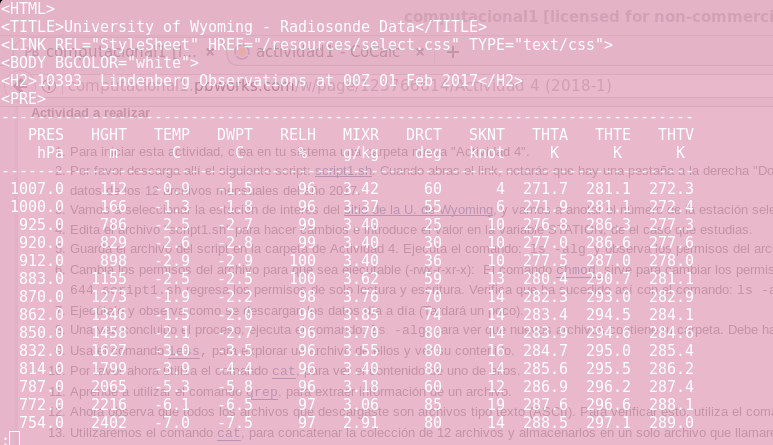
\includegraphics[width=0.8\textwidth]{less1.png}

Comando less

\end{center}

Siguiendo con la actividad se utilizó el comando \textbf{"cat"} par explorar un archivo, a diferencia del less, este te mostraba rapidámente el archivo y dejaba el puntero al final del archivo:
\begin{center}
 
\includegraphics[width=1\textwidth]{cat1.PNG}
 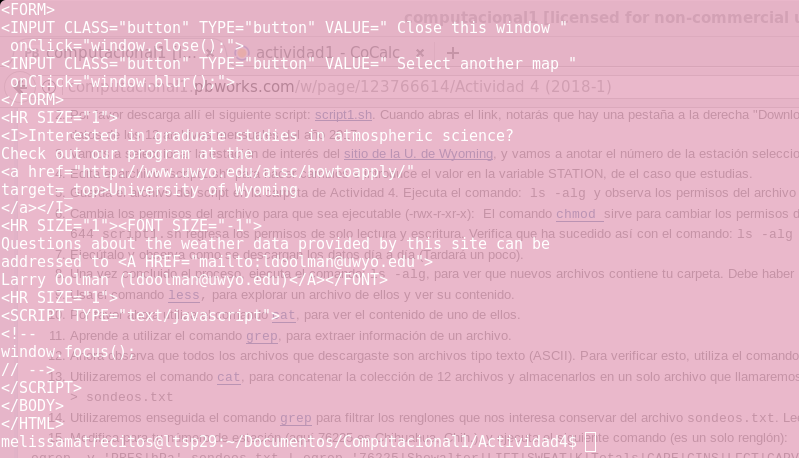
\includegraphics[width=0.8\textwidth]{cat2.png}

Comando cat

\end{center}

Otro comando utilizado fue el \textbf{"echo"}, el cual sirvió para escribir texto en un archivo, en este caso el archivo "file1":

\begin{center}
 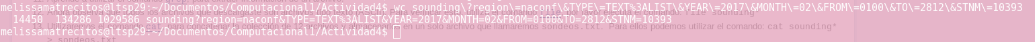
\includegraphics[width=1\textwidth]{echo.png}

Comando echo

\end{center}

También se utilizó el comando\textbf{"wc"}, con este contamos las palabras de un archivo:
\begin{center}
 
\includegraphics[width=1\textwidth]{wc.png}

Comando wc

\end{center}

Después se hizo uso del comando \textbf["grep"], el cual sirve para extraer información específica de los archivos. También se utilizó el comando \textbf{"file"} para para verificar que los archivos descargados fueran tipo ASCII.
Posteriormente se utilizó la instrucción:
\begin{verbatim} cat sounding* > sondeos.txt
\end{verbatim}
para almacenar los 12 archivos descargados en unos solo de nombre sondeos, aquí el redirector \textbf{">"} sirvió para enviar los 12 archivos al archivo nuevo, siguiendo con la practica se volvió a utilizar comando grep, luego se utilizó la siguiente entrada:
\begin{verbatim}
egrep -v 'PRES|hPa' sondeos.txt | egrep '10393|Showalter|LIFT|SWEAT|K|Totals|CAPE|CINS|LFCT|CAPV|Temp|Pres|thick|Precip' > df2017.csv
\end{verbatim}
la cual, selecciona solamente los renglones especificados, los cuales están separados por el rediccionador \textbf{"|"}, guardandolos en un archivo llamado "df2017.csv".
\begin{center}
 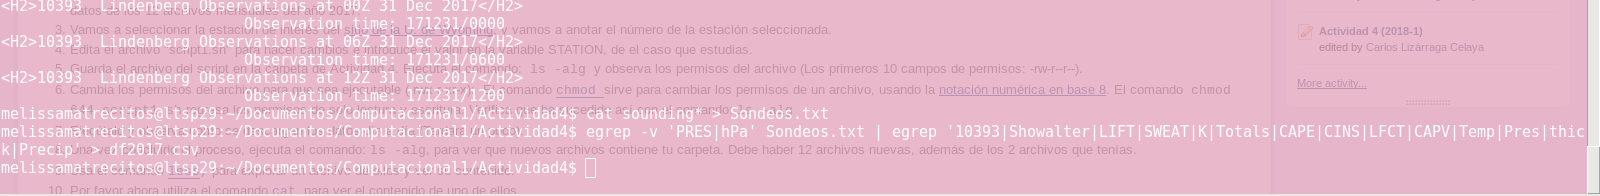
\includegraphics[width=1\textwidth]{egrep.png}

\end{center}
 Para automatizar el proceso anterior, se procedió a crear un script con los dos ultimos comandos utilizados, crear su ejecutable y ejecutarlo, solo "df2017.csv", fue enviado a "df2017-2.csv":
 \begin{center}
 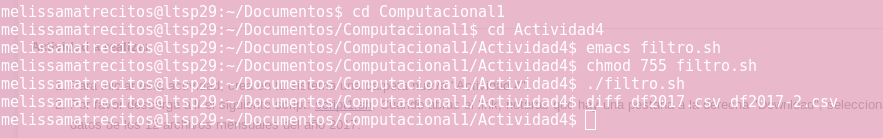
\includegraphics[width=0.8\textwidth]{egrepa.png}
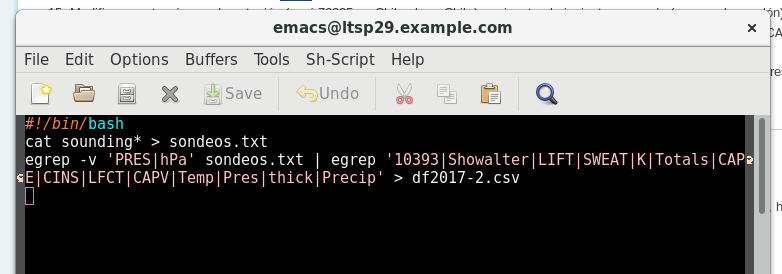
\includegraphics[width=0.8\textwidth]{egrepa2.png}
\end{center}

Por último se nos pidióo comparar estos dos archivos, lo cual se hizo con el comando \textbf{"diff"} y no se encontraron diferencias:
 \begin{center}
 
\includegraphics[width=1\textwidth]{diff.png}

\end{center}

\section{Conclusión}
Al inció de la actividad me pareció muy complicado entender que era lo que estábamos haciendo, pero conforme fui avanzando las dudas se resolvieron, descubriendo así muchas herramientas que ayudan en la optimización de procesos, sobre todo aquellos donde se tienen que trabajar con muchos datos.
\section{Bibliografía}
\begin{itemize}
\item Shell (computing). (2018). En.wikipedia.org. Recuperado el 20 Febrero 2018, de \url{https://en.wikipedia.org/wiki/Shell_(computing)}
\item Parker, S. (2017). Shell Scripting Tutorial. Shellscript.sh. Recuperado el 21 Febrero 2018, de \url{https://www.shellscript.sh/index.html}
\item Atmospheric Soundings. (2018). Weather.uwyo.edu. Recuperado el 21 Febrero 2018,de \url{http://weather.uwyo.edu/upperair/sounding.html}
\end {itemize}

\section{Apendice}
\begin{enumerate}
\item¿Qué fue lo que más te llamó la atención en esta actividad?

La manera tan sencilla en que se pueden automatizar procesos que manejan gran cantidad de datos  ya que solo conocía comandos muy básicos.

\item¿Qué consideras que aprendiste?

Como automatizar procesos por medio de scripts, así como los comandos que estos utilizan.

\item¿Cuáles fueron las cosas que más se te dificultaron?

Al inicio batallé mucho para saber que era lo que estaba haciendo, ya que no sabía para que eran los comandos. Creo que esto se debe a que un nuevo "lenguaje".

\item¿Cómo se podría mejorar en esta actividad?

Me hubiera gustado una introducción teórica a lo que íbamos  hacer, para no estar tan perdida y así poder agilizar el desarrollo de la actividad.

\item¿En general, cómo te sentiste al realizar en esta actividad?

Al inicio estaba muy confundida, pero al final me gustó mucho todo lo que hicimos.

\end{enumerate}

\end{document}
